\newpage
\subsection{Lukket kabinet}
Der blev først og fremmest set på karakteristikken for et helt lukket kabinet. Det vil altså sige, at alle propper blev sat over basreflekshullerne. Frekvenskarakteristikken blev herefter målt med CLIO Pocket lige foran membranen og i \SI{1}{\meter} afstand foran membranen. Resultatet af disse målinger ses på figuren nedenfor.\fixme{inkluder simulering i figuren. Derudover ville lidt teori om frekvenskarakteristikken for et lukket kabinet være lækkert, inden vi kaster os ud i målinger. Også så vi kan sammenholde teori med praksis -AB}
\begin{figure}[H]
	\centering
	\vspace{-12pt}
	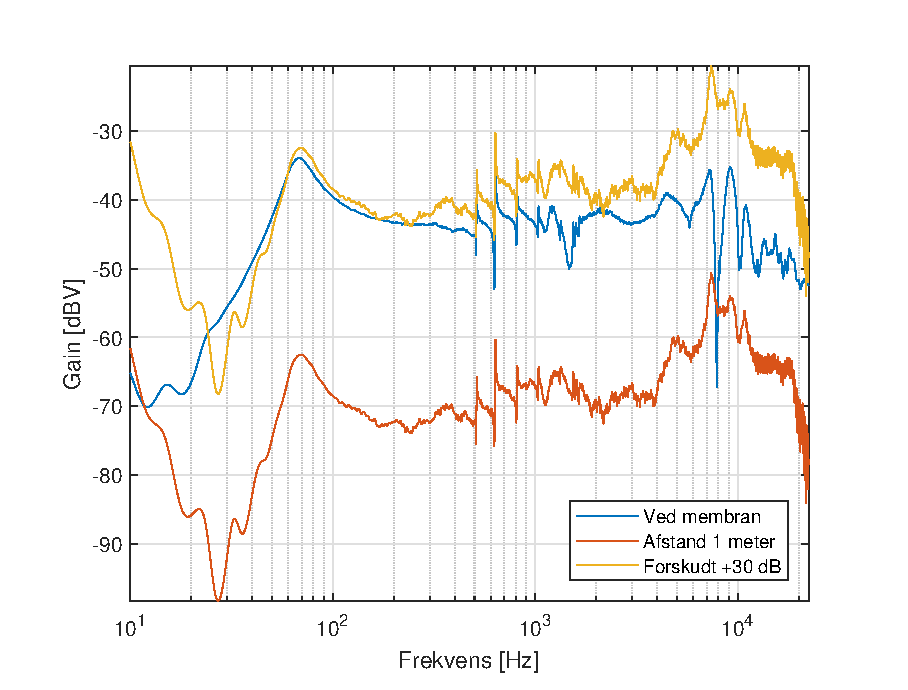
\includegraphics[width=\textwidth]{Billeder/Grafer/ClosedCabinet}
	\caption{Målinger på et lukket kabinet}
\end{figure}

Disse måleresultater udtaler sig som sagt ikke om hvordan basrefleksen påvirker frekvenskarakteristikken - men de vil blive brugt som referencemålinger i mange af de følgende måleopstillinger og resultater.

\begin{wrapfigure}{r}{0.5\textwidth} 
	\vspace{-20pt}
	\begin{center}
		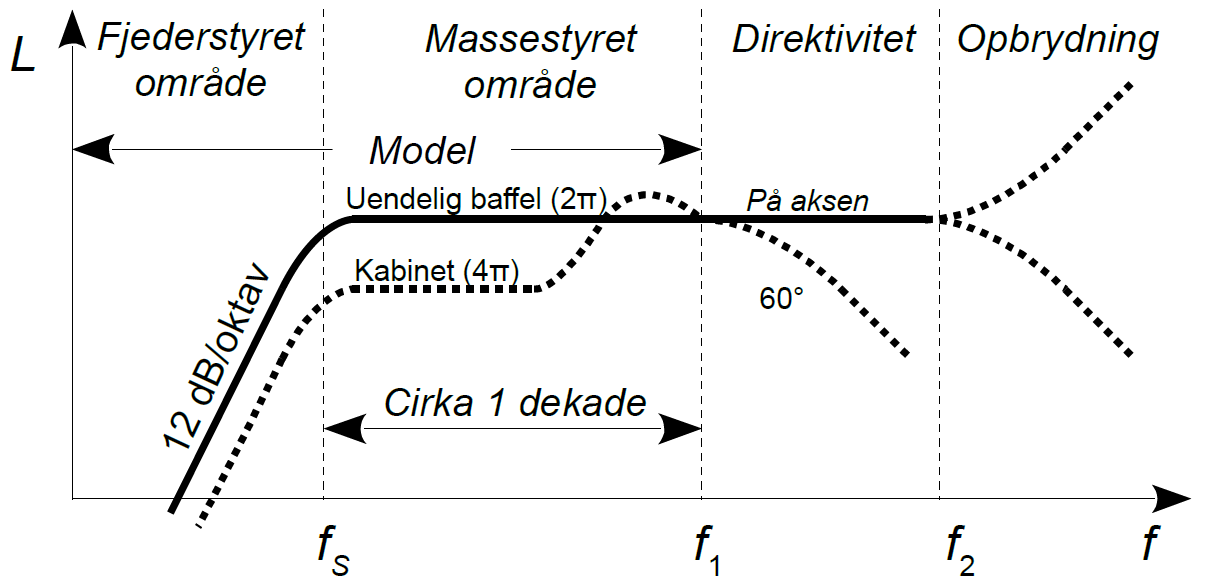
\includegraphics[width=0.5\textwidth]{Billeder/FrekvenskarakteristikTeori}
	\end{center}
	\vspace{-15pt}
	\caption{Teoretisk frekvenskarakteristik}
	\vspace{-20pt}
\end{wrapfigure}
På figuren ovenfor optræder nogenlunde den type karakteristik vi forventer. Det er især resonansfrekvensen $f_s$ ved \SI{70}{\hertz} som er meget interessant idet denne frekvens adskiller det \textbf{fjederstyrede område} fra det \textbf{massestyrede område}. Derudover er der blevet målt en hældning på kurven svarende til omkring +18 dB/oktav i det fjederstyrede område - altså en smule mere end den teoretiske stigning.

Hvis det, som omtalt i teorien, også antages at frekvensen $f_1$ ligger en dekade over $f_s$, så svarer denne frekvens altså til \SI{700}{\hertz}. Herefter vil direktiviteten begynde at spille en stor rolle på frekvenskarakteristikken.

På grafen ses det også, at når CLIO-mikrofonen flyttes længere væk fra membranen, så bevarer karakteristikken nogenlunde sin form i det massestyrede område og et godt stykke ind i både området over og under i frekvensspektret. Den største forskel er dog, at karakteristikken er blevet dæmpet med omkring -30 dB. Derfor er den ovenstående kurve målt i 1 meters afstand også blevet korrigeret med +30 dB for at vise dette. \fixme{Vi behøver vel ikke korrigere? Vi skal bare holde 1m afstand-måling sammen med 1m afstand, og tæt afstand med tæt afstand}

For at eftervise at dette er korrekt, så ses der på den nedenstående formel der giver en sammenhæng mellem lydtryk og afstand fra lydgiveren:
\begin{equation}
L_2 = L_1 - \left| 20 \cdot \log \left( \frac{r_1}{r_2} \right) \right|
\end{equation}

Hvor værdierne $L_1$ og $L_2$ er lydtryksniveauet målt i afstandene $r_1$ og $r_2$. Hvis der ses peaken omkring den første resonansfrekvens $f_s$, så ligger denne ved omkring $-\SI{34}{\decibel}$ når der måles tæt på højtaleren og $-\SI{62.5}{\decibel}$, når der måles i 1 meters afstand. Hvis disse værdier indsættes i den førnævnte formel, så findes der følgende:
\begin{equation}
\SI{-62.5}{\decibel} = \SI{-34}{\decibel} - \left| 20 \cdot \log \left( \frac{r_1}{\SI{1.00}{\meter}} \right)\right| \quad \Rightarrow \quad r_1 \approxeq \SI{3}{\centi\meter}
\end{equation}

Hvilket altså vil sige, at CLIO-mikrofonen har været placeret omkring \SI{3}{\centi\meter} fra højtaleren. Dette virker også meget sandsynligt.

Grunden til afvigelsen i det fjederstyrede område\fixme{ift hvad? - AB} kan skyldes, at dæmpningsfaktoren i luft er meget anderledes ved lave frekvenser\fixme{ref? - AB}. Afvigelsen ved de højere frekvenser skyldes at direktiviten spiller ind. Det kan derfor sagtens tænkes, at CLIO-mikrofonen ikke har stået præcist vinkelret ind på højtalerens midte. \fixme{Men netop de lavere frekvenser burde vel være ligeglade, da der her ikke spiller direktivitet ind (fjederstyret område) - AB}